\section{Vergleichswerkstoffe}
\label{sec:vergleichswerkstoffe}

\figref{fig:woehler_vergleich_werkstoffe} stellt die Läufe mit PA46-GF30 neben die 14 Läufe mit POM aus dem Jahr 2023 aus \secref{sec:versuchsprogramm}. Eingetragen sind nur Läufe bei der Referenzdrehzahl ihres Prüfstands, $3000$\,1/min am Rad auf dem Prüfstand KV3 und $2250$\,1/min auf dem Prüfstand KV4. Die Geraden stehen in \tabref{tab:vergleich_geraden}, angepasst wie in \secref{sec:woehlerlinien} mit der Untergrenze $0{,}10$ der Standardabweichung.

\begin{figure}[htbp]
    \centering
    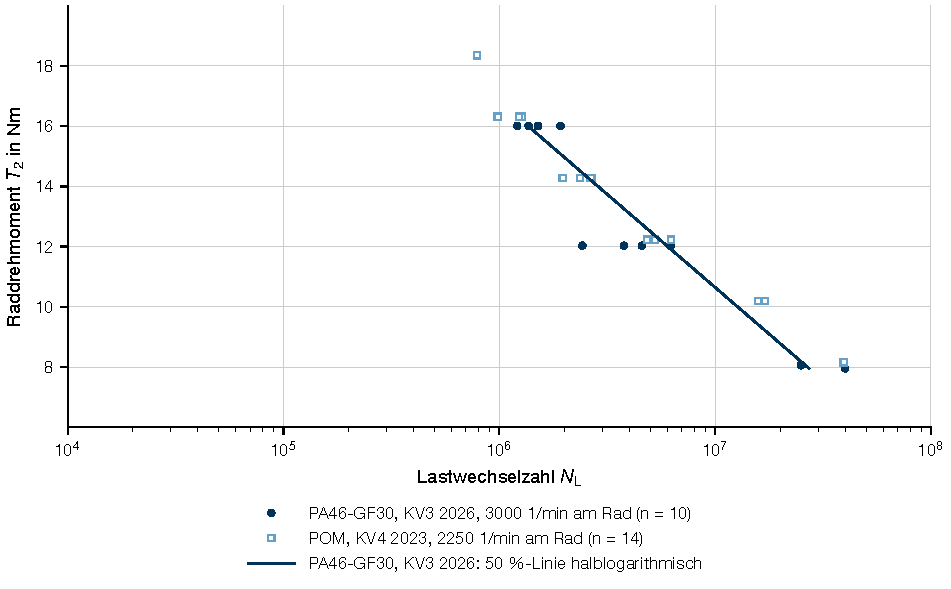
\includegraphics[width=\textwidth]{kap6/woehler_T2_vergleich_werkstoffe}
    \caption{Laufversuche mit PA46-GF30 (Prüfstand KV3, 2026, $3000$\,1/min, gefüllte Marker) neben POM (Prüfstand KV4, 2023, $2250$\,1/min, offene Marker) über dem Raddrehmoment, dazu die Gerade für $50$\,\% von PA46-GF30.}
    \label{fig:woehler_vergleich_werkstoffe}
\end{figure}

\begin{table}[htbp]
    \caption{Halblogarithmische Geraden $\lg N_{\mathrm{L},50\%} = a_{\mathrm{c}} - b_{\mathrm{c}} \, T_{2}$ von PA46-GF30 und POM mit der korrigierten Standardabweichung $s_{\lg N}$, dem Neigungsexponenten $k$ der doppeltlogarithmischen Geraden und dem belegten Bereich. $T_{2}$ in Nm.}
    \label{tab:vergleich_geraden}
    \centering
    \footnotesize
    \setlength{\tabcolsep}{4pt}
    \begin{tabular}{L{2.0cm}L{3.4cm}L{0.6cm}L{1.2cm}L{1.7cm}L{1.4cm}L{1.1cm}L{2.2cm}}
        Werkstoff & Prüfstand, Jahr, Drehzahl & $n$  & $a_{\mathrm{c}}$ & $b_{\mathrm{c}}$ in 1/Nm & $s_{\lg N}$ & $k$      & Bereich in Nm        \\
        \hline
        PA46-GF30 & KV3, 2026, $3000$\,1/min  & $9$  & $8{,}72$         & $0{,}162$                & $0{,}129$   & $4{,}40$ & $8$ bis $16$         \\
        POM       & KV4, 2023, $2250$\,1/min  & $14$ & $8{,}95$         & $0{,}176$                & $0{,}100$   & $5{,}20$ & $8{,}2$ bis $18{,}4$ \\
    \end{tabular}
\end{table}

Auf der Stufe $16$\,Nm erreichen die Räder aus PA46-GF30 $1{,}21$ bis $1{,}92 \cdot 10^{6}$ Lastwechsel, die Räder aus POM bei $16{,}3$\,Nm $0{,}98$ bis $1{,}27 \cdot 10^{6}$. Auf der Stufe $12$\,Nm liegen $3{,}8$ bis $6{,}2 \cdot 10^{6}$ Lastwechsel von PA46-GF30 im Bereich der POM-Räder bei $12{,}2$\,Nm mit $4{,}8$ bis $6{,}3 \cdot 10^{6}$. Bei $8$\,Nm stehen $25$ und geschätzt $40 \cdot 10^{6}$ Lastwechsel neben $39 \cdot 10^{6}$ des einen POM-Rades bei $8{,}2$\,Nm. Die Gerade von PA46-GF30 verläuft mit $b_{\mathrm{c}} = 0{,}162$\,1/Nm flacher als die von POM mit $0{,}176$\,1/Nm. Bei $16$\,Nm liegt sie um den Faktor $1{,}15$ über der POM-Geraden, bei $12$\,Nm gleichauf und bei $8$\,Nm um den Faktor $0{,}83$ darunter. Innerhalb der Streuung beider Reihen unterscheiden sich die Lebensdauern damit kaum. Den Vorteil der Faserverstärkung, den die Steifigkeit und die Zugfestigkeit des Werkstoffs erwarten lassen, zeigt dieser Vergleich nicht. Er steht allerdings unter Vorbehalt. Die POM-Räder liefen auf einem anderen Prüfstand mit einem anderen Ritzel, bei $2250$ statt $3000$\,1/min und mit $4{,}0$ statt $1{,}5$\,l/min Öl, und bei POM versagten die Räder nach Fiederling durch Zahnfußbruch nach schleichendem Risswachstum \cite[S.~66]{Fie23}, während die Räder aus PA46-GF30 nach \secref{sec:schadensbilder} eine Stufe der eingearbeiteten Ritzelkopfkante und aufgeraute Flanken tragen. Welcher dieser Einflüsse den Abstand trägt, lässt sich aus den Läufen nicht trennen. Die Läufe mit POM und PEEK auf dem Prüfstand KV3 im Jahr 2026 werden nach \secref{sec:pruefstand} nicht herangezogen.

% TK erledigt (nur POM 2023, Tabelle auf zwei Zeilen, Vorbehalte benannt): Bitte nochmal den gesamten Abschnitt Überarbeiten, auf aktuelle Informationene, die dir vorliegen und bitte gib mir Bescheid, wenn ich dir aus der Excel helfen soll, da ich einige Formulierungen im Text sehe, die darauf aufbauen, was wirklich aus der Excel ausgewertet wird. Da nicht ganz bekannt es, welches Peek früher gefarhen wurde, bitte nur die POM Läufe gegenüberstellen und auch nicht die POM Läufe von 2026. Also rein die von 2023 verwenden.

% Herkunft: 80_output/messungen/woehler/vergleich.md (POM KV4 2023 n = 14: a_c 8,9482, b_c 0,17639, s 0,0913 → 0,100,
%   k 5,199, 8,16 bis 18,35 Nm; Punkte kst-E_10 bis 41), woehler.md (PA46-GF30); Faktoren: 10^(8,721−0,1617·T) gegen
%   10^(8,9482−0,17639·T') mit T' = T·52/51 (16: 1,36e6/1,18e6 = 1,15; 12: 5,96e6/6,25e6 = 0,95; 8: 26,7e6/32,3e6 = 0,83);
%   Öldurchfluss 4,0 (2023, Fie23 S. 40) und 1,5 l/min (2026, kap3_2); Versagensart POM: MA-0296 S. 66.
